\documentclass{assignment}
\usepackage{arch_template} % Required for inserting images

\student{Natalie Chmura}
\semester{2024}
\date{\today}

\usepackage{tikz}
\tikzset{
  LabelStyle/.style = { rectangle, rounded corners, draw,
                        minimum width = 2em, fill = yellow!50,
                        text = red, font = \bfseries },
  VertexStyle/.append style = { inner sep=5pt,
                                font = \normalsize\bfseries},
  EdgeStyle/.append style = {->, bend left} }
\usetikzlibrary {positioning}
\usetikzlibrary{shapes}
\usetikzlibrary{automata}
\tikzset{
mystyle/.style={
  circle,
  inner sep=0pt,
  text width=6mm,
  align=center,
  draw=black,
  fill=white
  }
}


\courselabel{Individual Studies}
\exercisesheet{Research}{Minimum Spanning Tree Rotation Transforms}

\school{Arts and Sciences}
\university{\textbf{THE} Ohio State University}

\begin{document}

\begin{problem}

\section*{Preface}

\noindent The premise of this paper is to derive an algorithm  that finds the minimum number of right and left rotations that transforms one Binary Search Tree into a transformed version (Same nodes, different structure)

\subsection*{Background and Assumptions} \\

\begin{center}
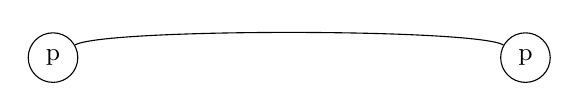
\begin{tikzpicture}
\small
    \node[mystyle] (1) at (-3, 0) {p};
    \node[mystyle] (2) at (3, 0)  {p};
    \draw (1) edge[out=30,in=150,looseness=0.2] (2);
\end{tikzpicture}
\end{center}


\end{problem}

\end{document}
